\documentclass{article}
\usepackage{../lambdatex} %disponibile all'indirizzo http://lambdamath.altervista.it/esercizi/lambdatex.sty
\usepackage{tasks}
\usepackage{exsheets}
\newcommand{\se}{\text{ se }}
\renewcommand{\phi}{\varphi}
\everymath{\displaystyle}

\title{Università degli Studi di Trento - Dipartimento di Matematica\\
CdL in Matematica – a.a. 2022–2023\\ Note esercitazione}
\author{Esercitatore: Simone Verzellesi\thanks{Trascrizione a cura di Davide Borra}}
\date{28 Novembre 2022}
\begin{document}
\maketitle
\lhead{Note esercitazione}
\chead{Università degli Studi di Trento - Dipartimento di Matematica\\
CdL in Matematica – a.a. 2022–2023}
\rhead{28/11/2022}
\setlength{\headheight}{30pt}
% \begin{question}
%     pippo
%\end{question}
\begin{enumerate}[label=\textbf{Esercizio 10.\arabic*.},itemindent=*]
%%%%%%%%%%%%%%%%%%%%%%%%%%%%%%%%%%%%%%%%%%%%%%%%%%%%%
\item Sia $f:[a,b]\to\R$ Riemann integrabile e $g: [a,b]\to \R$ limitata tali che \[f(x)=g(x)~~\forall x \in[a,b]\setminus \{x_0\}\]Dimostrare che $g$ è Riemann integrabile e che $\int_a^bf(x)dx=\int_a^bg(x)dx$.
\item[\textit{\large Soluzione~}]~
    \paragraph*{Ricorda}(linearità dell'integrale) $\phi, \psi\in \mathcal{R}([a,b])$ e $\alpha, \beta\in \R$
    \[\int_a^b(\alpha \phi+\beta\psi)dx=\alpha\int_a^b\phi dx+\beta \int_a^b\psi dx\]
\begin{proof}
    Non è restrittivo supporre $f(x_0)>g(x_0)$. Definiamo
    \[h(x):=f(x)-g(x)=\begin{cases}
        0&\se x\neq x_0\\
        f(x_0)-g(x_0)&\se x=x_0
    \end{cases}\]
    e dimostriamo che $h$ è Riemann integrabile. Equivalentemente dimostriamo che 
    \[\forall \varepsilon>0~~\exists \mathcal{D}:S(\mathcal{D},h)-s(\mathcal{D},h)<\varepsilon\]
    Fissiamo $\varepsilon$ e definiamo
    \[\mathcal{D}_\varepsilon=\left\{a,x_0-\frac{\epsilon}{4h(x_0)},x_0+\frac{\epsilon}{4h(x_0)}, b\right\}\]
    Si ottiene che 
    \[s(\mathcal{D}_\varepsilon, h)=0\]
    infatti l'$\inf$ di $h$ su qualsiasi intervallo è 0. Si ha inoltre che
    \[\begin{aligned}S(\mathcal{D}_\epsilon, h)&=\cancel{(x_1-a)\sup_{[a,x_1]}f}+(x_2-x_1)h(x_0)+\cancel{(b-x_2)\sup_{[x_2,b]}f}=(x_1-x_2)(h(x_0))=\\&=\left[\cancel{x_0}+\frac{\varepsilon}{4h(x_0)}-x_0+\frac{\varepsilon}{4h(x_0)}\right]h(x_0)=h(x_0)\frac{\varepsilon}{2h(x_0)}=\frac{\varepsilon}{2}<\varepsilon\end{aligned}\]
$h$ è quindi Riemann integrabile, di conseguenza per linearità $g=f-h$ è Riemann integrabile. Rimane ora da dimostrare che $\int_a^bf(x)dx=\int_a^bg(x)dx$. Dimostriamo equivalentemente che $\int_a^bh(x)dx=0$. Osserviamo che le somme inferiori sono sempre 0, mentre le somme superiori risultano limitate dall'alto da $\frac{\varepsilon}{2}$, quindi facendo tendere $\varepsilon$ a 0 si ottiene che 
\[0=s(\mathcal{D})\leq \int_a^bh(x)dx\leq \frac{\varepsilon}{2}\]
\[\implies \int_a^bh(x)dx=0\]
\end{proof}
%%%%%%%%%%%%%%%%%%%%%%%%%%%%%%%%%%%%%%%%%%%%%%%%%%%%%
\item Sia $f:[a,b]\to\R$ continua. Dimostrare che se $f(x)\geq 0 ~~\forall x  \in [a,b]$ e $\int_a^bf(x)dx=0$, allora $f(x)=0$ ovunque. 
\item[\textit{\large Soluzione~}]~
\begin{proof}
    Si procede per assurdo: supponiamo che $\exists x_0\in [a,b]:f(x_0)\neq 0$. In particolare $f(x_0)>0$ per ipotesi. Per il teorema della permanenza del segno \[\exists \delta >0:[x_0-\delta,x_0+\delta]\subseteq [a,b] \land f(x)>0~~\forall x\in [x_0-\delta,x_0+\delta]\]. Per lo spezzamento si ha\[\int_a^bf(x)dx=\int_a^{x_0-\delta}f(x)dx+\int_{x_0-\delta}^{x_0+\delta}f(x)dx+\int_{x_0+\delta}^bf(x)dx\geq \int_{x_0-\delta}^{x_0+\delta}f(x)dx\]
    Perchè gli altri due integrali sono non negativi per ipotesi.
    \[\int_{x_0-\delta}^{x_0+\delta}f(x)dx=\sup s(\mathcal{D},f)\geq2\delta \inf_{[x_0-\delta, x_0+\delta]}f=2\delta \inf_{[x_0-\delta, x_0+\delta]}f>0\]
    Poiché $\inf_{[x_0-\delta, x_0+\delta]}f=\min_{[x_0-\delta, x_0+\delta]}f>0$, ottengo una contraddizione.
\end{proof}
%%%%%%%%%%%%%%%%%%%%%%%%%%%%%%%%%%%%%%%%%%%%%%%%%%%%%
\item Scrivere i primi due termini dello sviluppo di Taylor centrato in $x_0=0$ della funzione
\[g(x)=\int_{x^3}^{-x^2}e^{-t^2}dt\]
E determinare per quali $\alpha$ reali 
\[\lim_{x\to0^+}\frac{g(x)}{x^\alpha}=0\]
\item[\textit{\large Soluzione~}]~
Definiamo 
\[f(x):=\int_0^xe^{-t^2}dt\]
Da cui
\[g(x)=\int_{x^3}^0e^{-t^2}dt+\int^{-x^2}_0e^{-t^2}dt=-\int^{x^3}_0e^{-t^2}dt+\int^{-x^2}_0e^{-t^2}dt=f(-x^2)-f(x^3)\]
Di conseguenza per il teorema fondamentale del calcolo integrale
\[g'(x)=f'(-x^2)(-2x)-f'(x^3)(3x^2)=-2xe^{-x^4}-3x^2e^{-x^6}\]
\[\implies g'(0)=0\]
\[g''(x)=-2e^{-x^4}+8x^4e^{-x^4}-6x{e^{-x^6}}+18x^7e^{-x^6}\]
\[\implies g''(x)=-2\]
Inoltre
\[g(0)=\int_{0}^{0}e^{-t^2}dt=0\]
Di conseguenza si ha \[g(x)=g(0)+g'(0)x+\frac{g''(0)}{2}x^2+o(x^2)=-x^2+o(x^2)\tag{$x\to0$}\]
Quindi
\[\lim_{x\to0^+}\frac{g(x)}{x^\alpha}=\lim_{x\to 0^+}\frac{-x^2+o(x^2)}{x^\alpha}=\lim_{x\to 0^+}\frac{x^2\left(-1+\frac{o(x^2)}{x^2}\right)}{x^\alpha}=\lim_{x\to 0^+}x^{2-\alpha}\left(-1+\frac{o(x^2)}{x^2}\right)=0~~\Harr~~\alpha<2\]
%%%%%%%%%%%%%%%%%%%%%%%%%%%%%%%%%%%%%%%%%%%%%%%%%%%%%
\item Sia 
\[g(x)=\int_0^{x^2}\cos(2t)dt\]
\begin{enumerate}
    \item trovare i punti critici di $g(x)$;
    \item calcolare 
    \[\lim_{x\to0^+}\frac{g(x)-x^2}{x^6}\]
\end{enumerate}
\item[\textit{\large Soluzione~}]~
\begin{enumerate}
    \item Sia $f(x)=\int_0^{x}\cos(2t)dt~~\implies~~g(x)=f(x^2)$. Di conseguenza $g'(x)=2xf'(x)=2xcos(2x^2)$. $x$ è punto critico $\Harr$
    \[\begin{cases}{ll}
        \Harr~& x=0\lor cos(2x^2)=0\\
        \Harr~& x=0\lor 2x^2=\frac{\pi}{2}+k\pi ~~~(k\in \Z)\\
        \Harr~& x=0\lor x=\pm\sqrt{\frac{\pi}{4}+k\frac{\pi}{2}} ~~~(k\in \N)
    \end{cases}\]
    \item ~\[\lim_{x\to0^+}\frac{g(x)-x^2}{x^6}=\left[\frac{0}{0}\right]\overset{\text{H}}{=}\lim_{x\to0^+}\frac{g'(x)-2x}{6x^5}=\lim_{x\to0^+}\frac{2x\cos (2x^2)-2x}{6x^5}=\lim_{x\to0^+}\frac{\cos(2x^2)-1}{4x^4}\frac{4}{3}=\frac{2}{3}\]
\end{enumerate}

%%%%%%%%%%%%%%%%%%%%%%%%%%%%%%%%%%%%%%%%%%%%%%%%%%%%%
\item Studiare qualitativamente 
\[F(x)=\int_{\frac{\pi}{4}}^{x}\cos(2t)dt\]
\item[\textit{\large Soluzione~}]~
Cominciamo rappresentando $\cos 2x$
\begin{figure}[ht]
    \centering
    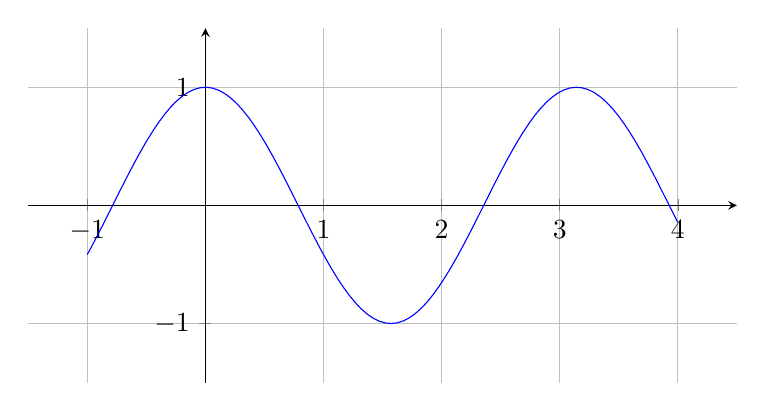
\begin{tikzpicture}
    \begin{axis}[
        x=1.5cm,y=1.5cm,
        axis lines=middle,
        ymajorgrids=true,
        xmajorgrids=true,
        xmin=-1.5,
        xmax=4.5,
        ymin=-1.5,
        ymax=1.5,
        xtick={-1.0,-0.0,...,4.0},
        ytick={-1.0,-0.0,...,1.0},]
        \draw [samples=100, domain=-1:4, color=blue] plot(\x,{cos(2*(\x*180)/pi)});
    \end{axis}
    \end{tikzpicture}
\end{figure}
Prima di tutto osserviamo che la funzione integrale ha una radice in $x=\frac{\pi}{4}$. Inoltre, spostandosi verso destra, tra $\frac{\pi}{4}$ e $\frac{\pi}{2}$ l'area è negativa e \textit{sempre più grande}. Di conseguenza la funzione integrale sarà decrescente e concava. Tra $\frac{\pi}{2}$ e $\frac{3}{4}\pi$ l'area sarà negativa (funzione integrale decrescente) e \textit{sempre più piccola} (convessa). Analogamente negli altri intervalli. Siamo così in grado di disegnare $F(x)$ in $\left[ \frac{\pi}{4}, \frac{5}{4}\pi\right]$. Siccome la funzione è periodica siamo quindi in grado di disegnare $F$ su tutto $\R$.
\begin{figure}[ht]
    \centering
    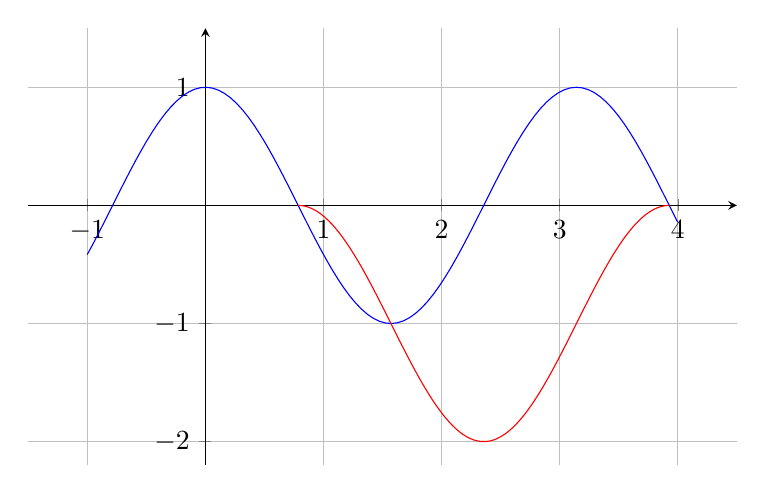
\begin{tikzpicture}
    \begin{axis}[
        x=1.5cm,y=1.5cm,
        axis lines=middle,
        ymajorgrids=true,
        xmajorgrids=true,
        xmin=-1.5,
        xmax=4.5,
        ymin=-2.2,
        ymax=1.5,
        xtick={-1.0,-0.0,...,4.0},
        ytick={-2.0,-1.0,...,1.0},]
        \draw [samples=100, domain=-1:4, color=blue] plot(\x,{cos(2*(\x*180)/pi)});
        \draw [samples=100, domain=pi/4:5*pi/4, color=red] plot(\x,{2*sin(2*(\x*180)/pi)/2-1)});
    \end{axis}
    \end{tikzpicture}
\end{figure}
%%%%%%%%%%%%%%%%%%%%%%%%%%%%%%%%%%%%%%%%%%%%%%%%%%%%%

\begin{table*}[ht]
    \centering
    \section*{Primitive elementari}
    \begin{tabular}{|m{0.2\textwidth}|m{0.2\textwidth}|}
        \hline\begin{center}\textbf{Funzione}\end{center} & \begin{center}\textbf{Primitiva}\end{center}\\ \hline\hline
        \[x^\alpha~~~~(\alpha\neq -1)\]& \[\frac{1}{\alpha+1}x^{\alpha+1}\]\\\hline
        \[\frac{1}{x}\]&\[\log|x|\]\\\hline
        \[e^x\]&\[e^x\]\\\hline
        \[a^x~~~(a>0\land a\neq 1)\]&\[\frac{a^x}{\log a}\]\\\hline
        \[\sin x\]&\[-\cos x\]\\\hline
        \[\cos x\]&\[\sin x\]\\\hline
        \[\sinh x\]&\[\cosh x\]\\\hline
        \[\cosh x\]&\[\sinh x\]\\\hline
        \[\frac{1}{\cos^2x}\]&\[\tg x\]\\\hline
        \[\frac{1}{1+x^2}\]&\[\arctg x\]\\\hline
        \[\frac{1}{\sqrt{1+x^2}}\]&\[\arcsin x\]\\\hline
        \[-\frac{1}{\sqrt{1+x^2}}\]&\[\arccos x\]\\\hline
    \end{tabular}
\end{table*}
\newpage
%%%%%%%%%%%%%%%%%%%%%%%%%%%%%%%%%%%%%%%%%%%%%%%%%%%%%
\item Calcolare i seguenti integrali indefiniti
\begin{tasks}(3)
    \task$\int\frac{3-4x}{1+x^2}dx$
    \task$\int\frac{1}{x\sqrt{1-\log^2x}}$
    \task$\int\sqrt[3]{2x+1}dx$
    \task$\int6x\sin(-3x^2-2)dx$
    \task$\int3xe^{x^2}dx$
\end{tasks}
\item[\textit{\large Soluzione~}]~
\begin{tasks}(1)
    \task$\int\frac{3-4x}{1+x^2}dx=3\int\frac{1}{1+x^2}dx-4\int\frac{x}{1+x^2}dx=3\arctg x-2\int\frac{2x}{1+x^2}dx=$\\$=3\arctg x-2\int \log'(1+x^2)2xdx=3\arctg x-2\int(\log(1+x^3))'dx=3\arctg x-2\log (1+x^2)+c$
    \task$\int\frac{1}{x\sqrt{1-\log^2x}}=\int \frac{1}{x}\arcsin'(log(x))dx=\int(\arcsin(\log x))'dx=\arcsin\log x+c$
    \task$\int\sqrt[3]{2x+1}dx=\frac{1}{2}\int 2(2x+1)^{\frac{1}{3}}dx=\frac{1}{2}(2x+1)^{\frac{4}{3}}\cdot{3}{4}+c=\frac{8}{3}\sqrt[3]{(2x+1)^4}+c$
    \task$\int6x\sin(-3x^2-2)dx=\int(-6x)(-\sin(-3x^2-2)dx=\cos (-3x^2-2)+c$
    \task$\int3xe^{x^2}dx=\frac{3}{2}\int2xe^{x^2}dx=\frac{3}{2}e^{x^2}+c$
\end{tasks}
%%%%%%%%%%%%%%%%%%%%%%%%%%%%%%%%%%%%%%%%%%%%%%%%%%%%%
\end{enumerate}
\end{document}
